% Chapter Template

\chapter{Data gathering and processing}
\label{Chapter2}
Data were sourced from several streams. The Icelandic Meteorological Office (IMO) provided measurements from weather stations across Iceland, NWP data were downloaded from the Copernicus Arctic Regional Reanalysis dataset (CARRA), and finally a land-elevation model was also provided by the IMO.

\section{Automatic Weather Station Data}

IMO provided measurements from \nStationsMin weather stations across Iceland. The measurements that met the filtering criteria began in \startDateVedur and ended in 2023. Of these \nStationsMin stations, \nVedurMin were from the IMO, with the anemometer at 10~m above ground, while the remaining \nVGMin stations were from \href{https://www.vegagerdin.is/}{the Icelandic Road and Coastal Administration (IRCA)}, with the anemometer at 6–7~m above ground \cite{vegagerdin_postur}. The locations of these weather stations are shown in Figure \ref{fig:aws_map}.

Data from these automatic weather stations (AWS) are stored in hourly files, which aggregate the original 10-minute files; measurement errors—unrealistic spikes known as “nails”—have been removed in most cases. Each record contains the following information: date and time; station number (convertible to coordinates using another dataset of Icelandic meteorological stations); average wind speed ($f$); wind gust ($f_g$); standard deviation of the wind gust; wind direction ($d$); and standard deviation of the wind direction.

These measurements began at the end of the 20th century with the installation of the first AWSs, and more stations have been added in subsequent decades.

\begin{figure}
    \centering
    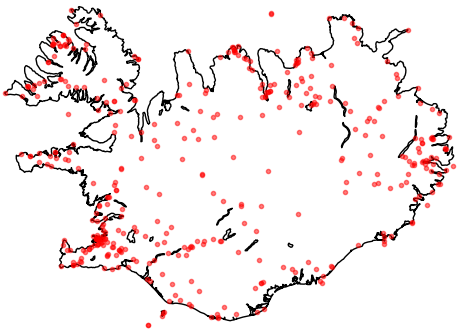
\includegraphics[scale = 1]{Figures/stationsOverIceland_2024-05-16_stripped_to_frame.png}
    \caption[Locations of automatic weather stations in Iceland]{Locations of all 412 stations that were looked at in this study. Most of these were from IMO but over a hundred were from IRCA. IMO anemometers are placed at 10 meters above ground, while IRCA ones are placed at 6--7 meters above ground.}
    \label{fig:aws_map}
\end{figure}

\section{CARRA Data}
CARRA is a high-resolution atmospheric reanalysis produced by the Copernicus Climate Change Service and run by ECMWF. It covers two regions, a west region covering Greenland and Iceland and an east region covering the European Arctic. It has a 2.5 km horizontal resolution and dates from 1991 to the present, with monthly updates. CARRA provides three-hourly analysis fields and short-term forecasts (hourly for lead times under 6 h and three-hourly beyond) of surface and near-surface variables—wind, temperature, pressure, precipitation, etc. It is based on the HARMONIE-AROME limited-area NWP model, forced at its boundaries by ERA5 (ECMWF Re-Analysis v. 5) and enhanced by local observations to better represent complex terrain, land–sea contrasts, and sea-ice processes. It is updated monthly, with a latency of 2-3 months\cite{carra_information}.

The CARRA dataset covers all the IMO observations that fulfill criteria of consistent availability – the oldest observation is from \startDateVedur. The CARRA-West region covers a vastly larger area than the area of interest. This leads to having to store a large amount of data. To download CARRA data one has two options, a web interface or using an API client provided by CARRA. Using the API client is the only realistic option here, as there are thousands of requests made for different times. If using the API, it is possible to query a smaller area (such as a rectangular area around Iceland) given a set of coordinates, but this is not possible with the web interface.

The requests to the API were made at each available CARRA hour ([00, 03, 06, 09, 12, 15, 18, 21]) on a grid covering Iceland, for each available observation time. The downloaded data were interpolated to get values at the weather stations. CARRA contains several types of layers: single levels, model levels, height levels, and pressure levels. The data for this thesis was downloaded from height levels. They were requested at heights of 15, 250 and 500 meters above ground. For each point 4 parameters were requested, wind speed, wind direction, pressure, and temperature.

\section{Elevation data}
A GeoTIFF file containing a digital elevation model (DEM) for Iceland on a 20~m by 20~m grid was provided by the Icelandic Meteorological Office (IMO). The entire country is covered by this file, and its size is approximately 685\,MB.

The Python package \texttt{rasterio} is used, enabling rapid elevation lookup via its spatial indexing and affine‐transform capabilities. Elevation at specified geographic coordinates can be retrieved directly, and grid indices may be used for efficient access. Elevation for any exact location can be interpolated by fetching neighboring grid points.

\section{Combining data sources}

Three main data sources were used, each requiring querying, filtering, and merging to prepare the combined dataset. When handling hundreds of thousands of rows, code efficiency is essential: row-by-row iteration can increase execution time dramatically compared to vectorized operations.

The sources were provided in different formats: IMO measurement data in text files, elevation data in GeoTIFF, and CARRA reanalysis data in GRIB. To train the models, these datasets were combined into a single file using the IMO measurements as a reference. CARRA data are supplied on a rectangular grid with approximately 2.5~km spacing, while IMO observations are tied to specific station locations. Elevation data are on a 20~m by 20~m grid covering Iceland. Linear interpolation was applied to merge the sources.

\begin{figure}[h]
  \centering
  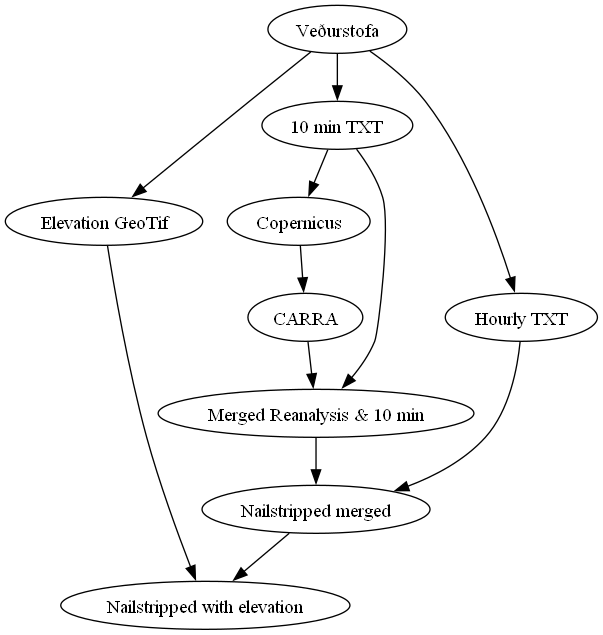
\includegraphics[scale=0.5]{Figures/data-preprocessing-flow-chart.png}
  \caption{Flow chart illustrating the data-combination workflow}
  \label{fig:data_preprocessing_flow_chart}
\end{figure}

The merging procedure, shown in Figure \ref{fig:data_preprocessing_flow_chart}, was as follows: for each AWS observation, a query was constructed for the CARRA API by specifying year, month, day, hour, and spatial extent. Because the API returns all specified days when queried by hour, and all specified months when queried by day, monthly queries were issued for only the required days, retrieving all eight three-hourly time points (00, 03, 06, 09, 12, 15, 18, and 21~UTC). After downloading the requested variables at the desired pressure levels, point values were interpolated and appended to a pandas dataframe. The monthly GRIB files were then discarded before proceeding to the next month. This strategy reduced storage needs from several terabytes to under one gigabyte.

Elevation values from the GeoTIFF were interpolated in the same manner: the four surrounding grid points were used in a linear interpolation to estimate the elevation at each station location. These interpolated values were included in the dataframe, since topography influences both average wind speed and gustiness \cite{GNP_vidtal}.

\section{Comparison of observed and reanalysis wind speed}

Differences between reanalysis and measured wind speeds can be substantial. Absolute error increases with wind speed, while percentage error decreases. An overview of these errors by wind-speed range is shown in Table \ref{table:measuredVSReanalysis_wind_speed}.

\begin{table}[h]
  \centering
  \caption[Measured vs.\ reanalysis wind-speed errors]{Comparison of measured and reanalysis wind speeds using mean absolute error (MAE) and mean absolute percentage error (MAPE). Values for observed wind speeds below 1~m/s are excluded to avoid inflated MAPE values. Measured speeds are at 10~m above ground (IMO) or 6–7~m (IRCA); reanalysis speeds are at 15~m.}
  \label{table:measuredVSReanalysis_wind_speed}
  \begin{tabular}{cccc}
    \toprule
    $f$ & $n$ & MAE & MAPE \\
    \midrule
    $[1; 5[$     & 5,260,814  & 2.0 & 83.9\% \\
    $[5; 10[$    & 4,150,923  & 2.2 & 31.3\% \\
    $[10; 15[$   & 1,480,487  & 2.5 & 21.0\% \\
    $[15; 20[$   &   388,905  & 3.0 & 17.8\% \\
    $[20; 25[$   &    84,099  & 4.0 & 18.4\% \\
    $[25; \infty[$ &   20,288 & 6.6 & 23.0\% \\
    $[1; \infty[$  &11,385,516 & 2.2 & 53.7\% \\
    \bottomrule
  \end{tabular}
\end{table}

Next, the distribution of MAE by station is examined, considering station location and number of observations. Figure \ref{fig:station_mae_distribution} shows this distribution, and Table \ref{table:station_mae_distribution} lists the five stations with the lowest MAE and the five with the highest MAE.

\begin{figure}[h]
  \centering
  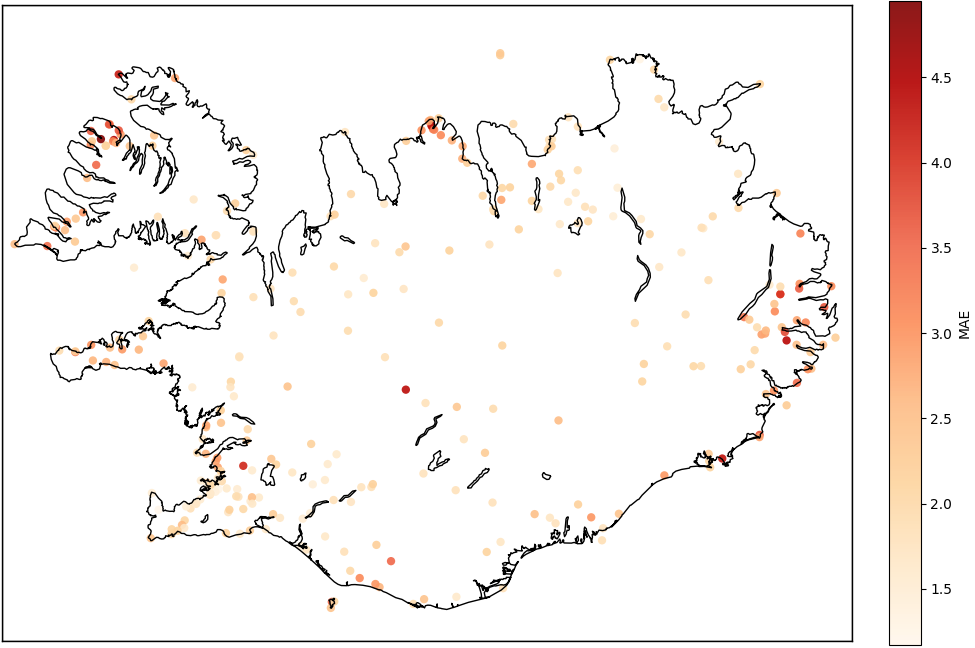
\includegraphics[scale=0.6]{Figures/MAEoverIceland.png}
  \caption[MAE distribution by station]{Distribution of mean absolute error (MAE) by station for all observed wind speeds.}
  \label{fig:station_mae_distribution}
\end{figure}

\begin{table}[h]
  \centering
  \caption[Station MAE extremes]{Mean absolute error (MAE) between reanalysis and observed wind speeds at the five stations with lowest and highest errors.}
  \label{table:station_mae_distribution}
  \begin{tabular}{lcc}
    \toprule
    Station               & $n$     & MAE  \\
    \midrule
    Reykjavík Háahlíð     & 6,800   & 1.17 \\
    Keflavíkurflugvöllur  & 52,000  & 1.18 \\
    Reykjavík Víðidalur   & 14,000  & 1.23 \\
    Rif á Melrakkasléttu  & 13,000  & 1.29 \\
    Reykjavíkurflugvöllur & 56,000  & 1.29 \\
    \midrule
    Almannaskarð          &  4,000  & 4.30 \\
    Kerlingarfjöll        & 15,000  & 4.36 \\
    Fáskrúðsfjarðargöng   &  7,900  & 4.40 \\
    Seljalandsdalur       &  1,600  & 4.51 \\
    Botn í Súgandafirði   & 32,000  & 4.95 \\
    \bottomrule
  \end{tabular}
\end{table}

\section{Layout of combined data}

Once data from all three sources have been retrieved and processed—including interpolation—they must be combined and formatted for modeling (training, validation, and testing). The starting point is a DataFrame containing AWS observations: average wind speed, wind gust, wind direction, station number, and coordinates. CARRA data are provided at selected height levels, each as a separate row in the CARRA DataFrame. Thus a single observation will span multiple rows, one per level. These rows are merged by time and station location, enabling AWS and CARRA data to be joined on station and time fields.

The DEM elevation data are handled by defining an upwind sector: a range of angles relative to the wind direction $d$ and radial distances from each station. Points within this sector are generated as shown in Code Listing \ref{code:sectorElevation}.

\begin{lstlisting}[
    style=Python,
    basicstyle=\small\ttfamily,
    caption={Generation of elevation points in the upwind sector},
    label=code:sectorElevation
]
angles = [(angle + (90 - d)) * pi/180 for angle in angleRange]
length_rng = [(exp(i * log(n + 1)/ k) - 1) * 1000 
              for i in range(1, k + 1)]
points = np.array([[(X + l * cos(angle), Y + l * sin(angle))
                    for angle in angles] for l in length_rng])   
\end{lstlisting}

The resulting DataFrame includes AWS measurements (our target), CARRA weather variables, and elevation points. An example of the combined data structure is shown in Table \ref{table:trainDataExample}.

\begin{table}[h]
    \centering
    \caption[Example of combined data structure]{Example of the combined data structure of features used for modeling. Data include derived variables Richardson number (Ri) and squared Brunt–Väisälä frequency ($N^2$), station altitude (meters above sea level), transformed wind direction (twd), wind speed (ws$_{15}$), wind direction (wd$_{15}$), temperature ($t_{15}$), pressure ($p_{15}$) (CARRA values at 15 m height), and elevation points (from DEM) in a sector pointing upwind.}
    \label{table:trainDataExample}
    \resizebox{\textwidth}{!}{
    \begin{tabular}{ccccccccccc}
        \toprule
        Ri & $N^2$ & \shortstack{station\\altitude} & twd & ws$_{15}$ & wd$_{15}$
        & $t_{15}$ & $p_{15}$ & $\text{elevation}_0$ & elevation$_1$ & \dots\\
        \midrule 
        -1.18 &  26700 & 100 & 1.5 & 10 & 5 & 0 & 100 & 2 & 4 & \dots\\
        \dots\\
        \bottomrule
    \end{tabular}
    }
\end{table}

The transformed wind direction is a proxy showing whether the wind is coming from land or sea. It is computed as the angle between the wind direction and a vector from the center of Iceland to the station.

The Richardson number and the Brunt–Väisälä frequency describe atmospheric stability, see equations (\ref{eqn:Ri}) and (\ref{eqn:N})  \cite{richardson_number_skybrary,brunt_vaisala_freq_eumtrain,mean_gust_HA_HO}. These values are calculated using reanalysis data at two different height levels. Thus Ri refers to the Richardson number calculated between height levels 15m and 500m. Exactly the same notation is used with the Brunt–Väisälä frequency, except the square is used.
%
\begin{equation}
  \label{eqn:Ri}
  Ri = \frac{g \cdot dT \cdot dz}{T_{\textrm ave} \cdot dU^2} \unit{[]}
\end{equation}
%
\begin{equation}
  \label{eqn:N}
  N = \sqrt{\frac{g \cdot dT }{T_{\textrm ave} \cdot dz}} \unit{[Hz]}
\end{equation}
%
Here, $g$ is gravitational acceleration; $dT$ the temperature difference between levels; $dz$ the height difference; $T_{\mathrm{ave}}$ the average temperature; and $dU$ the wind-speed difference. Lower Ri indicates greater turbulence, with typical values between 0.1 and 10, and values below 1 signifying significant turbulence \cite{richardson_number_skybrary}. Negative $N^2$ denotes instability, as an air parcel will accelerate away from its original position \cite{brunt_vaisala_freq_eumtrain}.

Since Ri and $N^2$ are derived from reanalysis variables, they add limited new information compared to the raw data, but they can reduce input dimensionality and improve model explainability via Shapley-value analysis \cite{shapley_information}. Shapley values assess feature importance by evaluating all possible feature subsets—an operation of computational complexity $2^n$. In practice, approximations are used but can still be costly for large models. Because $dU$ appears squared in the denominator of Ri, if the wind-speed difference between levels is very small, Ri can become arbitrarily large, potentially distorting predictions.

\section{Distributions of observed and reanalysis data}

CARRA reanalysis data may exhibit bias or systematic differences when compared to measurements. Figure \ref{fig:obs_carra_wind_speeds} shows the distributions of observed and reanalysis wind speeds. Although the shapes are similar, reanalysis values tend to be higher.

\begin{figure}[ht]
  \centering
  \begin{subfigure}[b]{0.8\textwidth}
    \centering
    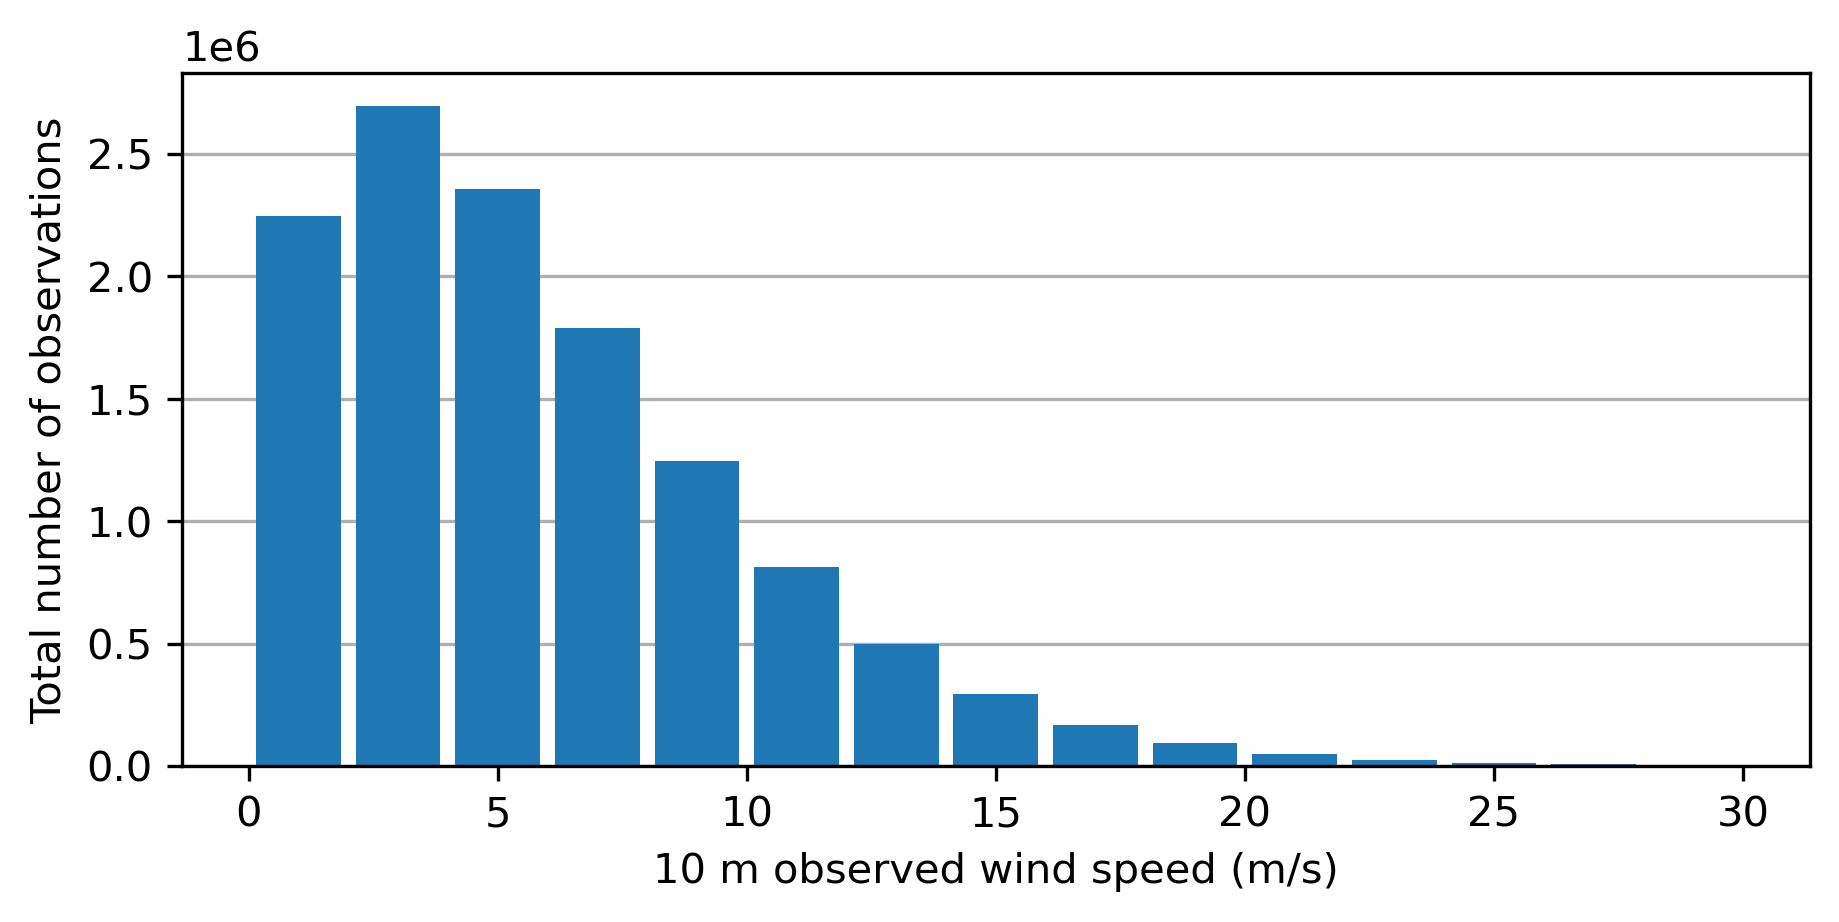
\includegraphics[width=\textwidth]{Figures/obs_wind_speeds.png}
    \caption{Histogram of observed wind speeds from IMO and IRCA at all stations, sampled at 3-hour intervals (00,~03,~06,~…~,21~UTC).}
    \label{fig:obs_wind_speeds}
  \end{subfigure}
  
  \vspace{0.5cm}
  
  \begin{subfigure}[b]{0.8\textwidth}
    \centering
    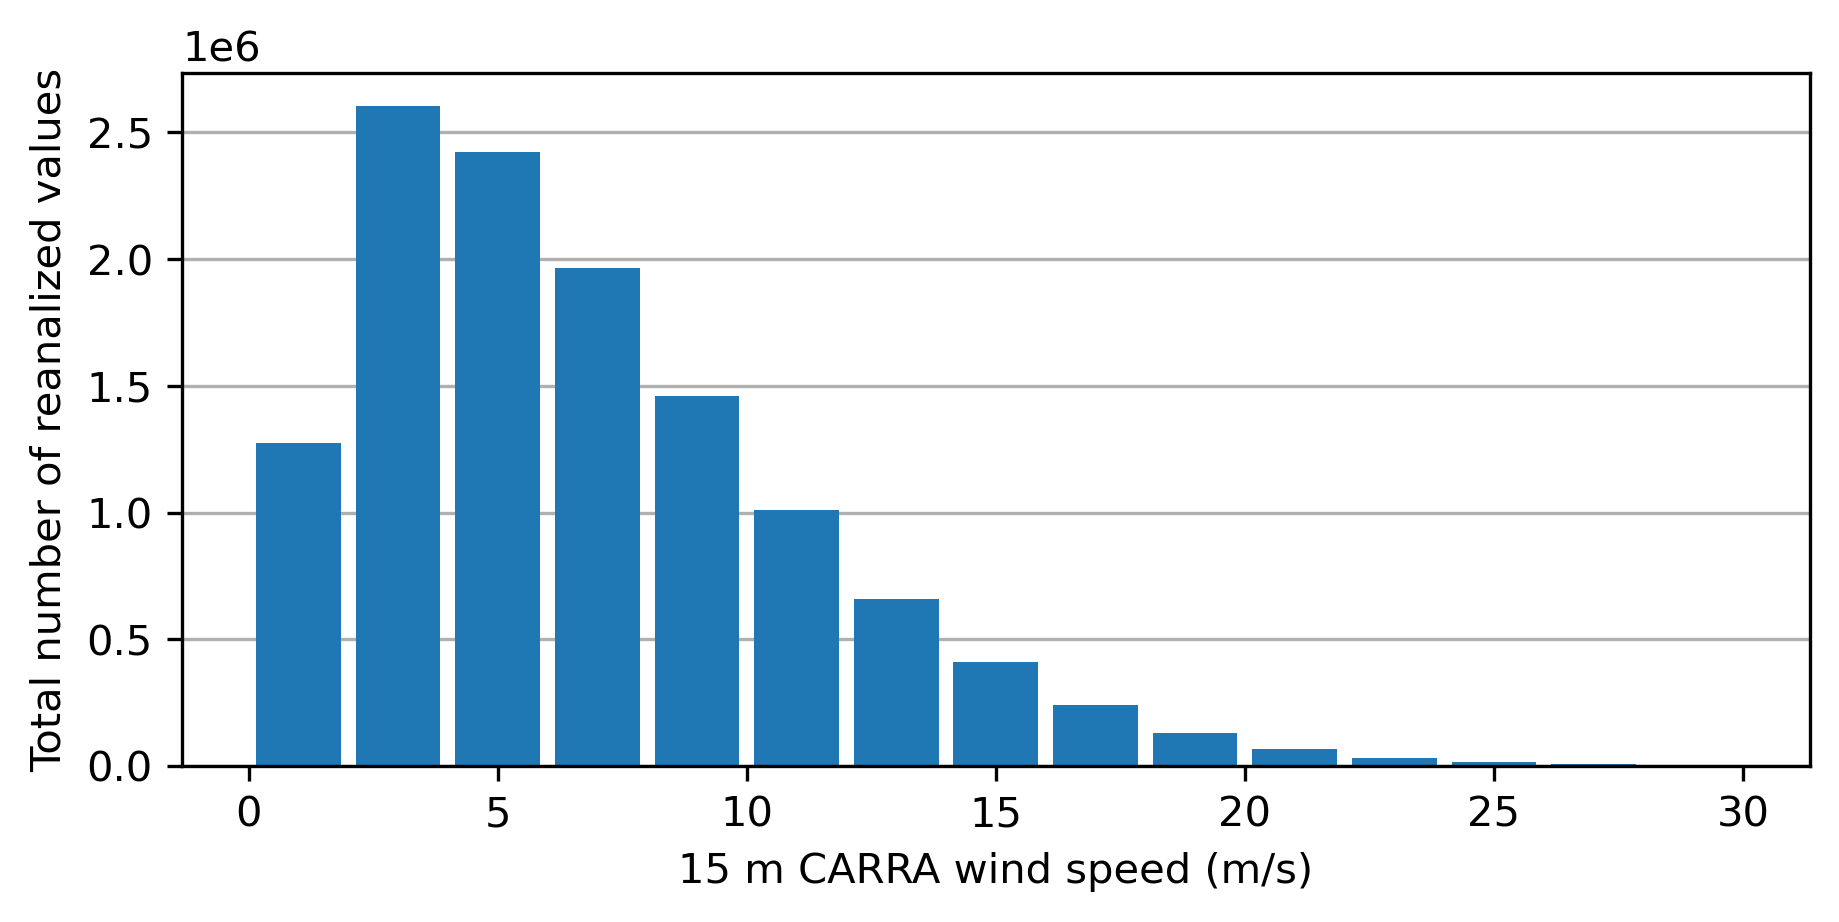
\includegraphics[width=\textwidth]{Figures/carra_wind_speeds.png}
    \caption{Histogram of interpolated CARRA wind speeds at station locations on a 2.5~km grid and 3-hour intervals.}
    \label{fig:carra_wind_speeds}
  \end{subfigure}
  
  \caption{Comparison of observed and reanalysis wind-speed distributions. CARRA values are spatially interpolated by linear weighting of surrounding grid points.}
  \label{fig:obs_carra_wind_speeds}
\end{figure}

\begin{figure}[ht]
  \centering
  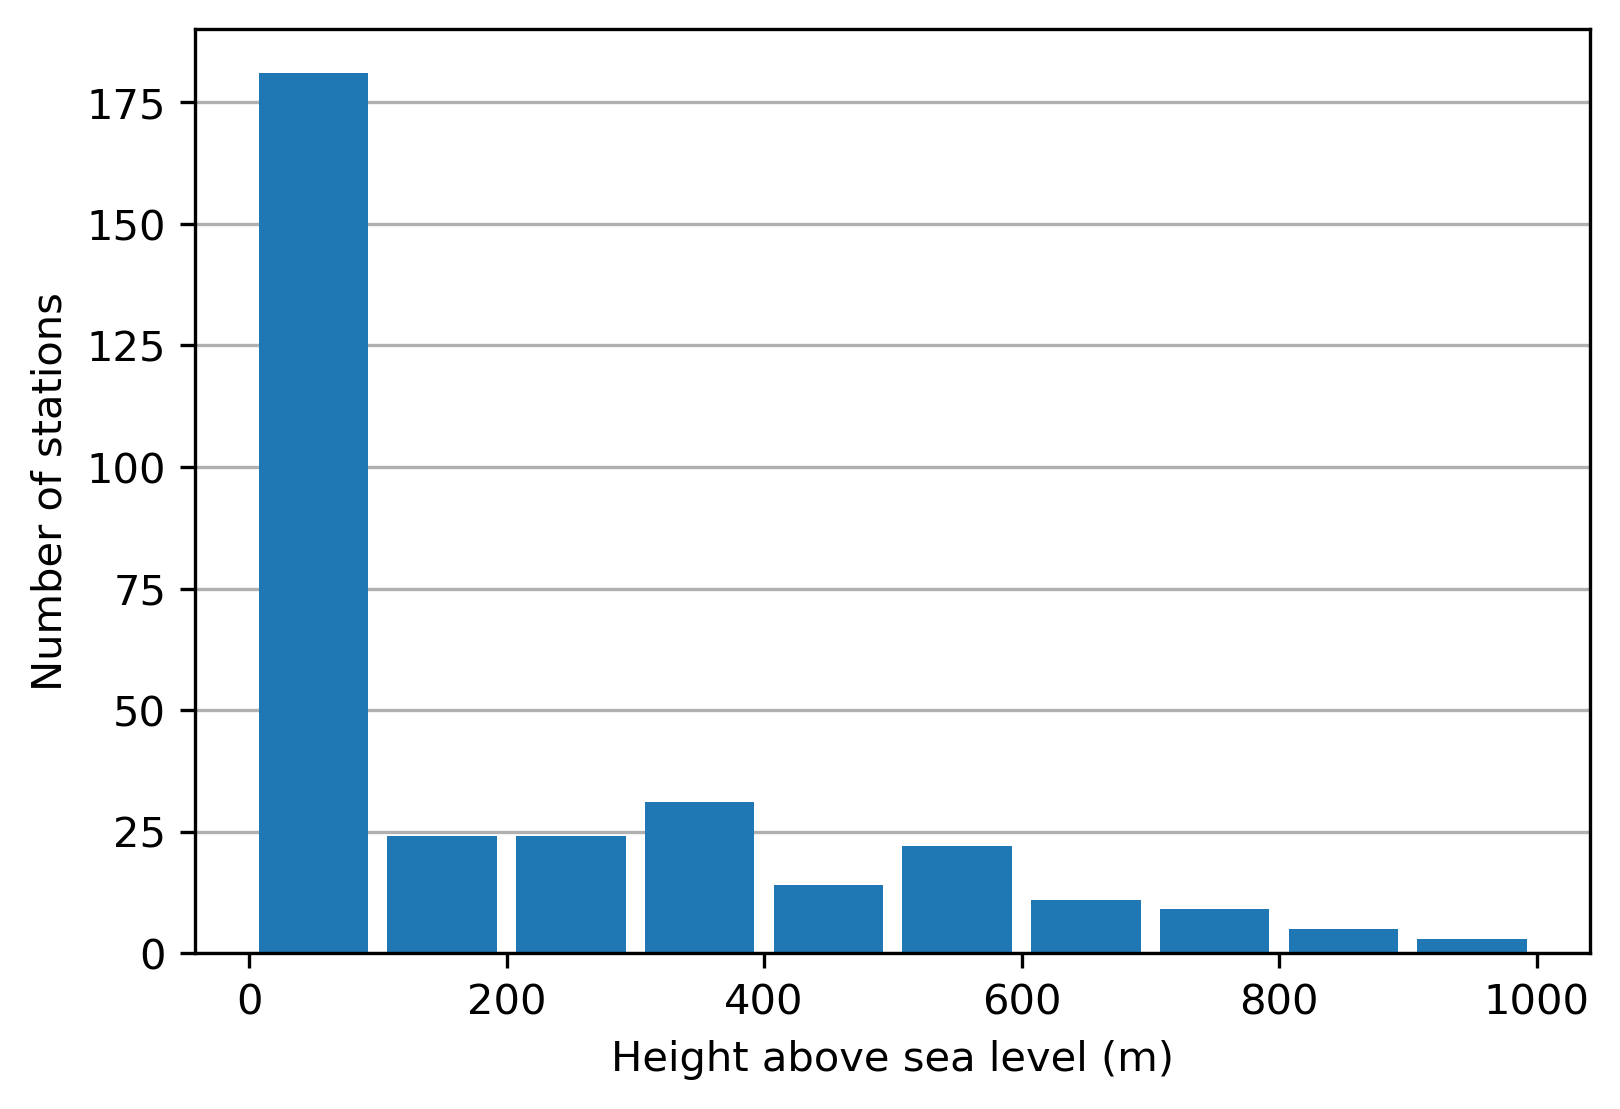
\includegraphics[width=0.8\textwidth]{Figures/station_heights.png}
  \caption{Distribution of weather station altitudes above sea level. One outlier near 2000~m was excluded due to limited and inconsistent data.}
  \label{fig:station_heights}
\end{figure}

\begin{figure}[ht]
  \centering
  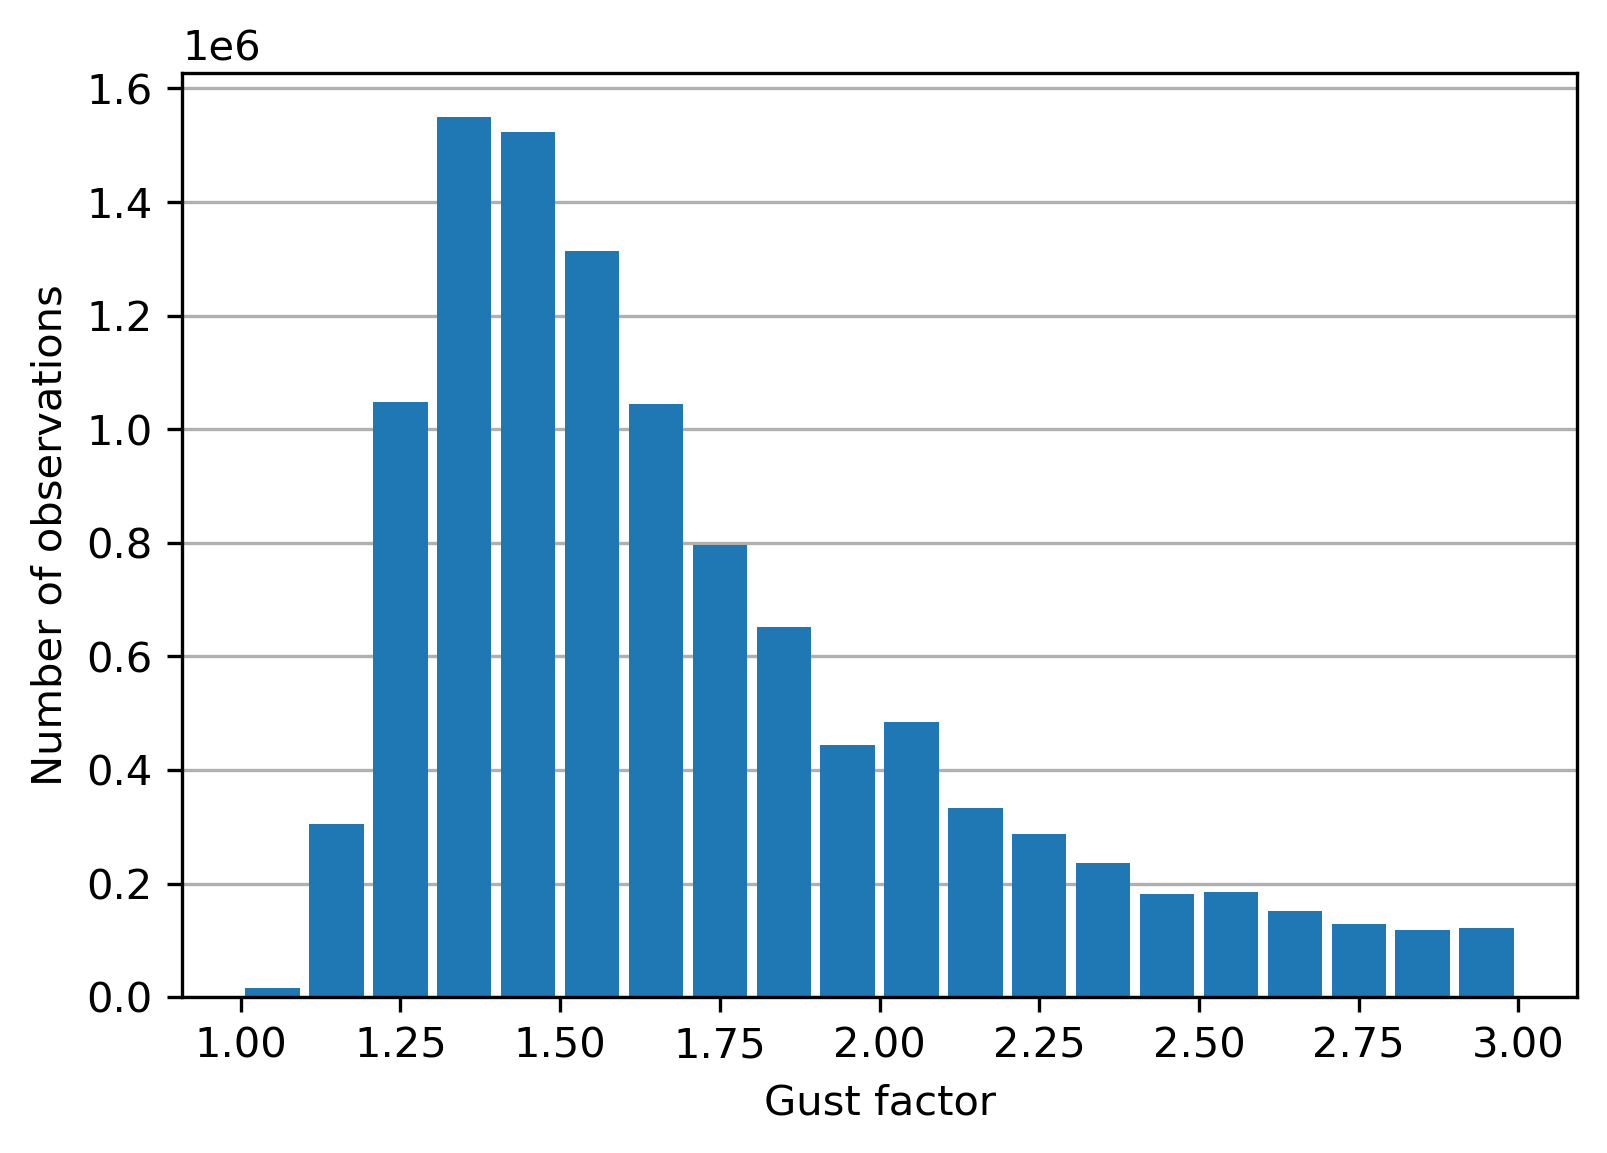
\includegraphics[width=0.8\textwidth]{Figures/gust_factor_2025.png}
  \caption{Histogram of gust factors. By definition, gust factor $\ge1$; most values lie between 1.2 and 2. The gust factor declines as wind speed increases.}
  \label{fig:gust_factors}
\end{figure}
